% ----------------------------------------------------------
% The Pipeline Algorithm
% ----------------------------------------------------------
\chapter{The Pipeline Algorithm}
\label{chapter:algorithm}

\SSSAY{Presentation of chapter}

\section{Extending the PDD flow for Pipelined Processors}

The Property-Driven Design flow presented on Sec.~\ref{subsection:PDD-flow} can be extended to help the hardware designer to deal with pipelined processors. Fig.~\ref{fig:new-pdd-flow} shows on its left side the original PDD flow. On the right side, an extended PDD flow is presented with two additional steps that are included to support pipelined processors; insert stages and pipeline algorithm. 

\begin{figure}[htb!]
	\centering
	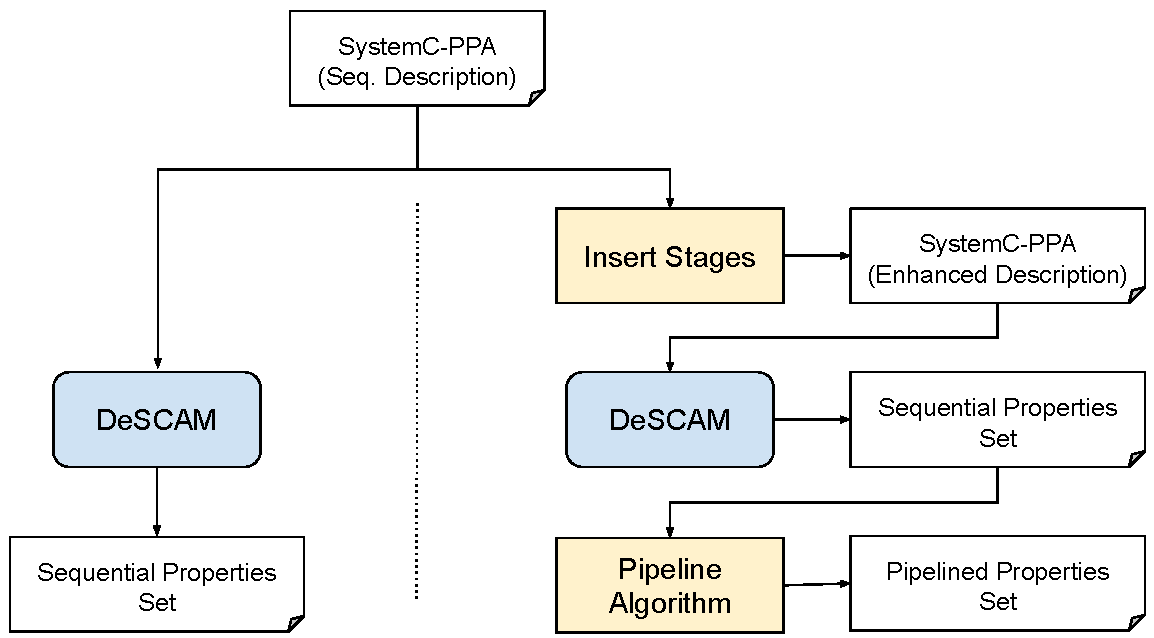
\includegraphics[width=0.85\textwidth]{images/new_pdd_flow.pdf}
	\caption{On the left, property generation with \textit{DeSCAM} for the original PDD flow. On the right, extension of the PDD flow to better support of pipelined processors.}
	\label{fig:new-pdd-flow}
\end{figure}

In the same manner as the original flow, the extended PDD flow starts with a description at the architectural-level, which is PPA compliant. Before applying the description to the \textit{DeSCAM} tool, the SystemC-PPA model is modified to include information about the pipeline behaviour resulting in an enhanced PPA description. This description can be applied to \textit{DeSCAM} which will generate a Sequential Property Set of \textit{micro properties} (to be detailed later in this section). Finally, the \textit{Pipeline Algorithm} can merge the \textit{micro properties} generating a Property Set with \textit{pipeline properties}.

The \textit{Insert Stages} phase allows the designer to include information about the desired pipeline structure into the SystemC-PPA model. It is important to emphasise that the designer does not have to translate the concurrent pipeline behaviour from the RTL implementation into the ESL model. The designer needs simply to include information about the desired pipeline stages at the appropriate points. This is done by calling the function \textit{insert\_state()} at the points in the data path of the ESL model corresponding to each pipeline stage. This function call will not influence on the sequential behaviour of the simulation for the model at the system-level.

The \textit{insert\_state()} function is interpreted by the \textit{DeSCAM} tool as a directive to include an important state in the PPA for that respective position in the code. Without this directive, the important states were only generated for communication calls, which affects the \textit{I/O} behaviour (see Sec.~\ref{subsection:PDD-flow}). Consider the regular PPA in Fig.~\ref{subfig:ppa-seq} extracted from a sequential ESL model without the manually inserted stages. If a call to insert a state for each pipeline stage is used, the resulting enriched PPA such the one in Fig.~\ref{subfig:ppa-pipe-processor} is obtained.

\begin{figure}[htb!]
\centering
\begin{subfigure}[b]{0.45\textwidth}
  \centering
	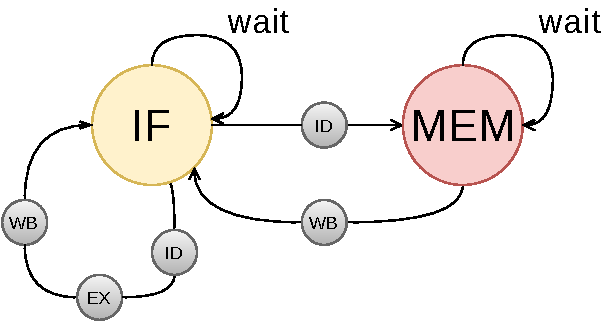
\includegraphics[width=0.9\textwidth]{images/PPA_old.pdf}
	\caption{PPA for regular PDD flow.}
	\label{subfig:ppa-seq}
\end{subfigure}
\hfill
\begin{subfigure}[b]{0.45\textwidth}
  \centering
	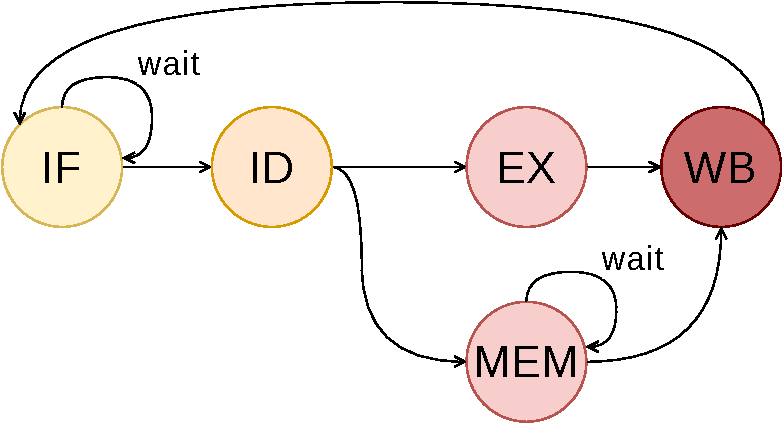
\includegraphics[width=0.9\textwidth]{images/PPA_new.pdf}
	\caption{PPA for extended PDD flow.}
	\label{subfig:ppa-pipe-processor}
\end{subfigure}
\caption{(a) PPA for a sequential SystemC-PPA processor description like in Fig.~\ref{fig:ppa-seq}. (b) Enriched PPA for an enhanced SystemC-PPA processor description with states inserted for each pipeline stage.}
\label{fig:ppa-old-and-new}
\end{figure}

The enriched PPA of Fig.~\ref{subfig:ppa-pipe-processor} derived from an enhanced SystemC-PPA has one important state for each pipeline stage. As a result, the property set generated by \textit{DeSCAM} will also be different. Let us consider an \textit{ADD} operation for a 4-stage pipeline processor as an example. The property generated by \textit{DeSCAM} for a regular sequential SystemC-PPA description is seen in the listing of Fig.~\ref{fig:ex-pdd-add-ppt}. Since only one important state, for instance \textit{IF}, is present on the execution path of an \textit{ADD} instruction, only one property is generated for describing the behaviour of this instruction. This can be also seen on the PPA of Fig.~\ref{subfig:ppa-seq} where the \textit{ADD} operation corresponds to a single edge starting on important state \textit{IF} and also ending at this important state. On the other hand, an \textit{ADD} instruction execution on the enriched PPA of Fig.~\ref{subfig:ppa-pipe-processor} corresponds to four edges. Therefore, four properties will be generated for this single instruction. These operations describing the behaviour between two pipeline stages are named \textit{micro operations}, or \textit{micro properties}. The listing on Fig.~\ref{fig:ex-two-micro-ppt} shows two examples of micro properties. The property in Fig.~\ref{subfig:ex-two-micro-ppt-if} corresponds to the operation between the \textit{IF} and \textit{ID} stages, and the property in Fig.~\ref{subfig:ex-two-micro-ppt-id} the operation when the IUV goes from stage \textit{ID} to \textit{EX}.

\begin{figure}[htb!]
     \centering
     \begin{subfigure}[b]{\textwidth}
         \begin{lstlisting}
    property PDD_ADD_IF;
    dependencies: no_reset;
    for timepoints:
        t_end = t+1;
    freeze:
        PC_at_t = PC@t;
    assume:
        at t: IF;
    prove:
        at t_end: ID;
        at t_end: PC == PC_at_t + 4;
        at t_end: fetched_instr == instr_in_sig;
        at t_end: operands == getOperandsFromRegFile(fetched_instr);
        during [t+1, t_end-1]: instr_req_out_notify == false;
        at t_end: instr_req_out_notify == true;
        during [t+1, t_end]: data_req_out_notify == false;
    end property;\end{lstlisting}
         \caption{Micro property describing operation from \textit{IF} stage to \textit{ID} stage.}
         \label{subfig:ex-two-micro-ppt-if}
     \end{subfigure}
     \hfill
     \begin{subfigure}[b]{\textwidth}
         \begin{lstlisting}
    property PDD_ADD_ID;
    dependencies: no_reset;
    for timepoints:
        t_end = t+1;
    freeze:
        PC_at_t = PC@t,
        fetched_instr_at_t = fetched_instr@t;
    assume:
        at t: ID;
        at t: getInstrType(fetched_instr) == ADD;
    prove:
        at t_end: EX;
        at t_end: PC == PC_at_t;
        at t_end: fetched_instr == fetched_instr_at_t;
        at t_end: ex_regData == operands.rs1 + operands.rs2;
        at t_end: ex_regAddr == operands.rd;
        at t_end: ex_regWrEn == true;
        during [t+1, t_end]: instr_req_out_notify == false;
        during [t+1, t_end]: data_req_out_notify == false;
    end property;\end{lstlisting}
         \caption{Micro property describing operation from \textit{ID} stage to \textit{EX} stage.}
         \label{subfig:ex-two-micro-ppt-id}
     \end{subfigure}
        \caption{Example of micro properties generated for an \textit{ADD} instruction from an enhanced SystemC-PPA processor description with states inserted to each pipeline stage. The property in (a) refers to the transition between \textit{IF} and \textit{ID} stages, and the property in (b) the transition between \textit{ID} and \textit{EX}.}
        \label{fig:ex-two-micro-ppt}
\end{figure}

One problem with describing the behaviour of a single instruction with multiple micro properties is that it becomes less intuitive for the designer. It is more natural to describe an instruction behaviour spawning over all pipeline stages. A second problem is that each micro operation generated will describe the behaviour of all \textit{outputs} and visible registers. As discussed in Sec.~\ref{section:pdd-pipe-processor}, this makes the property set impossible to hold because each property, in this pipelined processor context, should prove only the values of interest for the corresponding stage. An example of this problem can be observed in the micro properties of Fig,~\ref{fig:ex-two-micro-ppt}. The PC behaviour is correctly proven to be incremented in (a) when the IUV is on the \textit{ID} stage. However, in (b), the PC is proven to remain with the same value. This is not true as the PC is normally incremented in every clock cycle as a new instruction is fetched. Another inconsistency refers to the output signal requesting a new instruction, \textit{instr\_req\_out\_notify}. In the  commitments of (b), the signal is proven to be de-asserted, which is not the expected behaviour of a pipeline processor that requests a new instruction every clock cycle when there is no \textit{stall}.

The other additional phase included on the extended PDD flow of Fig.~\ref{fig:new-pdd-flow} is the \textit{Pipeline Algorithm}. This proposed algorithm combines the micro properties referring to a single instruction into a \textit{pipeline property} that comprises the behaviour of the instruction executing throughout all pipeline stages, similarly to the property shown in the listing of Fig.~\ref{fig:ex-add-ppt}. The Pipeline Algorithm is detailed in Sec.~\ref{sectio:pipe-algorithm}.

The notion of completeness discussed in Sec.~\ref{section:ipc-pipe-processor} and Sec.~\ref{section:s2qed} still applies. The set of pipeline properties generated by the algorithm represents the set of constrained properties that considers the IUV executing in a empty pipeline. For passing the case-split test and achieving completeness, a set of \SSQED{} properties has to be written.

Finally, in addition to the HDL template that can be generated by \textit{DeSCAM} in order to assist the designer on the RTL implementation, see Sec.~\ref{subsection:PDD-flow}, a new plugin  for \textit{DeSCAM} was developed in this work. This plugin can be optionally used by the designer to automatically generate a top design in HDL creating the environment to prove the \SSQED{} properties. The plugin is detailed in Sec.~\ref{section:plugio-s2qed-top}.

\section{The Algorithm}
\label{sectio:pipe-algorithm}

\section{The Plugin}
\label{section:plugio-s2qed-top}

\textcolor{red}{Will this be a chapter or a section? Both algorithm plugin and s2qed skeleton plugin here?}